\documentclass[11pt]{article}
\usepackage[T1]{fontenc}
\usepackage[english]{babel}
\usepackage{graphicx}
\usepackage{palatino}
\usepackage{helvet}
\usepackage{times}
\usepackage{layout}
\usepackage[a4paper,top=2.0cm, right=2.0cm, bottom=2.0cm, left=2.0cm]{geometry}
\usepackage{enumitem}
\usepackage{amsthm}
\usepackage{url}
\usepackage{multicol,caption}

\setlist{nolistsep}

\usepackage{fancyhdr}
\pagestyle{fancy}
\lhead{{\hvnb Colm}}
\chead{}
\rhead{}
\lfoot{}
\cfoot{}
\rfoot{}

\newcommand*{\helvetica}{\fontfamily{phv}\selectfont}
\newcommand*{\helveticanarrow}{\fontfamily{phv}\fontseries{mc}\selectfont}
\newcommand*{\hvnb}{\fontfamily{phv}\fontseries{bc}\selectfont}
\newcommand*{\palatino}{\fontfamily{ppl}\selectfont}
\newcommand*{\timesroman}{\fontfamily{ptm}\selectfont}

% Commands to produce formatted layout
\newcommand*{\projecttitle}[1]{\begin{center}\Large\hvnb{\color{blue} #1}\end{center}}
\newcommand*{\theauthor}[1]{\noindent  \helveticanarrow{#1}\\}



% Support for multiple bibliographies
\usepackage[sectionbib,numbers]{natbib}
\usepackage{chapterbib}

\usepackage[compact]{titlesec}
\usepackage{lipsum}
\usepackage{xcolor}
\usepackage{amsmath}
\usepackage{amsfonts}

\DeclareMathOperator*{\argmax}{arg\,max}
\DeclareMathOperator*{\argmin}{arg\,min}

\titleformat{\section}
  {\large\hvnb\color{blue}}{\thesection}{1em}{}
\titleformat{\subsection}
  {\hvnb}{\thesubsection}{1em}{}
\titleformat{\chapter}
  {\Large\hvnb\color{blue}}{Lecture \thechapter:}{1em}{}

\newenvironment{Figure} 
  {\par\medskip\noindent\minipage{\linewidth}}
  {\endminipage\par\medskip}

\newcommand{\pd}[2]{\frac{\partial #1}{\partial #2}}
\newcommand{\dd}[2]{\frac{d {#1}}{d {#2}}}
\DeclareMathOperator{\sgn}{sgn}

\begin{document}
\setlength{\bibsep}{0.2pt}
\setlength{\itemsep}{0.2pt}

\helveticanarrow
\rhead{\hvnb  23/07/2023 LML working notes}

\projecttitle{The $\eta$-compounding random walk}

%\theauthor{Colm Connaughton} 


\begin{multicols}{2}

\section{Appendix - binomial sums}
We will need finite sums of powers weighted by binomial coefficients:
\begin{align}
\label{eq:binomialSums} S_k(T) =  \sum_{n=0}^T {T \choose n}\,n^k,
\end{align}
which are essentially the moments of the binomial distribution with $p=\frac{1}{2}$. 
For $k=0$ we have $S_0(T) = 2^T$ from the  definition of the binomial distribution.
For $k\geq 0$, we can evaluate the sums sequentially by differentiating the binomial theorem,
\begin{align*}
(x+ y)^T =  \sum_{n=0}^T {T \choose n} x^n y^{T-n}
\end{align*}
with respect to $x$ and setting $x=y=1$.
For example, differentiating once with respect to $x$, we get
\begin{align*}
T \, (x+y)^{T-1} =  \sum_{n=0}^T {T \choose n} n x^{n-1} y^{T-n}
\end{align*}
and setting $x=y=1$ gives $S_1(T)$. We can now differentiate again and use the formula for $S_1(T)$ to get $S_2(T)$ and so on. 
The first few sums are:
\begin{align}
\label{eq:binomialSum0} \sum_{n=0}^T {T \choose n} =& 2^T\\
\label{eq:binomialSum1}  \sum_{n=0}^T {T \choose n} \,n  =& \sum_{n=0}^T {T \choose n} \,(T - n) = T\,2^{T -1}\\
\label{eq:binomialSum2}  \sum_{n=0}^T {T \choose n} \,n^2  =& \sum_{n=0}^T {T \choose n} \,(T - n)^2 = T\,(T+1)\,2^{T -2}.
\end{align}

\section{Definition of $\eta$-compounding}
Adopting the notation in \cite{yamano2002some} to fit the way we usually write the isoelastic utility function, we define the generalised exponential and logarithm as
\begin{align}
\label{eq:exp_eta}
\exp_\eta (x) = & \left\{
\begin{array}{ll} 
\left( 1 + (1-\eta)\,x\right)^\frac{1}{1-\eta} & \text{$0 \leq \eta < 1$}\\
\exp(x) & \text{$\eta=1$}
\end{array}
\right. \\
\label{eq:log_eta}
\log_\eta (x) = & \left\{
\begin{array}{ll} 
\frac{1}{1-\eta}\left( x^{1-\eta} -1 \right) &  \text{$0 \leq \eta < 1$}\\
\log(x) & \text{$\eta=1$}
\end{array}
\right. .
\end{align}
Following \cite{carr2022generalized} we define the generalised compounding operator, $\otimes$, as
\begin{align}
x \otimes y = & \exp_\eta\left[ \log_\eta(x )+ \log_\eta(y)\right].
\end{align}
An $\eta$-compounding process with growth factor, $g$, is one where the initial value is $\eta$-compounded by $g$ at each step:
\begin{align}
x_{t+1} =& x_t \otimes g,
\end{align}
with $x_0 = X_0$. For $T\geq 1$, we have
\begin{align}
\nonumber x_T = & X_0 \otimes  \underbrace{  g\otimes \ldots \otimes g}_{T\text{-times}}\\
\nonumber =&  X_0 \otimes \exp_\eta \left[  \underbrace{  \log_\eta(g)+ \ldots + \log_\eta(g)}_{T\text{-times}}\right]\\
\label{eq:deterministic}=& X_0 \otimes \exp_\eta\left[\log_\eta(g)\,T \right].
\end{align}
From this we see that the growth rate (the quantity with a dimension of $\text{time}^{-1}$) is $\log_\eta(g)$. From Eq.~(\ref{eq:exp_eta}), we see that $\exp_\eta(x)$ is only well defined for
\begin{align*}
x \geq & -\frac{1}{1-\eta} &  \text{$0 \leq \eta < 1$}\\
x >  & -\infty & \text{$\eta=1$}.
\end{align*}
Hence, for general values of $\eta \neq 1$, Eq.~(\ref{eq:deterministic}) is only well-defined for all $T \geq 1$ if $\log_\eta(g) >0$. This implies that $g\geq 1$. 
Some confusion can arise for some rational values of $\eta$ for which the branch point of Eq.~(\ref{eq:exp_eta}) at $x = -\frac{1}{1-\eta}$ disappears. 
For example, if $\eta=\frac{1}{2}$, we have
\begin{align*}
x_T =& \exp_\frac{1}{2}\left[\log_\frac{1}{2}(X_0) + T \log_\frac{1}{2} (g)\right]\\
=& \left[ \sqrt{X_0} + \frac{T}{2}\,\log_\frac{1}{2} (g) \right]^2.
\end{align*}
Although this is well defined for all $T$ even when $\log_\frac{1}{2} (g) <0$, it is not continuously reachable from $\eta = \frac{1}{2} \pm \epsilon$.
Furthermore, this results in an unnatural model where a negative growth rate corresponds to increasing $x_T$. 
In what follows we will respect the constraint $g \geq 1$ in order to avoid such pathologies.


\section{The $\eta$-compounding random walk}
We are interested in studying the $\eta$-compounding random walk in discrete time. At each step, there are now two possible growth factors, $g+r$ and $g-r$, which  we assume occur with equal probability: 
\begin{align}
\label{eq-etaRandomWalk}
x_{t+1} = \left\{ 
\begin{array}{ll}
x_t \otimes \left(g +r \right) & \text{with probability $\frac{1}{2}$}\\
x_t \otimes \left(g - r \right)  & \text{with probability $\frac{1}{2}$}.
\end{array}
\right.
\end{align}
with $x_0 = X_0$.
In order to keep everything well-defined we need $g-r > 1$, assuming that $g>0$ and $r>0$.

We can generalise some of the calculations for the multiplicative random walk in \cite{redner1990random} to the $\eta$-compounding random walk.  
If, after playing $T$ rounds of the game, we experience $n$ ``wins" (and $T-n$ "losses"), then $x_T$ will take the value
\begin{align*}
x_T =  &X_0\otimes \underbrace{(g+r)\otimes \ldots \otimes (g+r)}_{n\text{-times}} \otimes \underbrace{(g-r)\otimes \ldots \otimes (g-r)}_{T-n\text{-times}} \\
=& X_0\otimes\exp_\eta\left[n\,\log_\eta(g+r)\right] \otimes \exp_\eta\left[(T-n)\,\log_\eta(g-r) \right]\\
=& X_0\otimes \exp_\eta\left[ n\,\log_\eta(g+r) + (T-n)\log_\eta(g-r) \right].
\end{align*}
The probability of this value is
\begin{align}
\label{eq:binomialDistr}
p(n) = {T \choose n} \left(\frac{1}{2}\right)^T,
\end{align}
where ${T \choose n}$ is the binomial coefficient -  the number of ways in which $n$ wins can occur in a sequence of $T$ rounds of the game.
The expectation value of $x_T$ is therefore
\begin{align}
\nonumber \mathbb{E}\left[x_T \right] =& \sum_{n=0}^T  {T \choose n} \left(\frac{1}{2}\right)^T  X_0\otimes\exp_\eta\left[ n\,\log_\eta(g_1) \right.\\
\nonumber & \left. + (T-n)\log_\eta(g_2) \right]\\
\label{eq-expectationxT}=&   \frac{1}{2^T} \sum_{n=0}^T  {T \choose n} \left[X_0^{1-\eta } -T + n g_1^{1-\eta }+ (T-n) g_2^{1-\eta }\right]^{\frac{1}{1-\eta }},
\end{align}
where, for brevity we have written $g_1 = g+r$ and $g_2 = g-r$.

\section{Expectation value for the case of $\eta=\frac{1}{2}$}
This sum can be done exactly at least for the case $\eta = \frac{1}{2}$:
\begin{align}
\label{eq:expectationExact} \mathbb{E}\left[x_T\right] =& \frac{1}{4}\left(\sqrt{g+r}+\sqrt{g-r}-2\right)^2\,T^2 \\
\nonumber &+ \left[ (\sqrt{g+r}+\sqrt{g-r}-2) \sqrt{X_0} \right.\\
\nonumber & \left.+ \frac{1}{4}(\sqrt{g+r}-\sqrt{g-r})^2\right]\,T\\
\nonumber &+ X_0.
\end{align}
For large  $T$ we find
\begin{align}
\label{eq:ExLargeT}
\mathbb{E}\left[x_T \right]  \sim & \frac{1}{4} \left( \sqrt{g+r} + \sqrt{g-r} -2\right)^2\, T^2.
\end{align}

\section{Typical value for the $\eta$-compounding random walk}
The {\em typical} value of $x_T$ can be found by finding $n^*$,  the value of $n$ that maximises the probability, Eq.~(\ref{eq:binomialDistr}). This is
\begin{align*}
n^* =& \argmax_{n} {T \choose n}\\
=& \frac{T}{2}.
\end{align*}
Thus the typical value of $x_T$ is
\begin{align}
\nonumber \widetilde{x}_T =& X_0\otimes\exp_\eta\left[ \frac{T}{2}\,\left(\log_\eta(g+r) +\log_\eta(g-r)\right)\right]\\
\label{eq:typicalxT} =&\left(\text{X}_0^{1-\eta} + \left((g+r)^{1-\eta }+(g-r)^{1-\eta }-2\right)\, \frac{T}{2} \right)^\frac{1}{1-\eta}.
\end{align}
For large $T$, we find
\begin{align}
\widetilde{x}_T \sim & \left(\frac{1}{2}  \left((g+r)^{1-\eta }+(g-r)^{1-\eta }-2\right)\right)^\frac{1}{1-\eta} \, T^\frac{1}{1-\eta}.
\end{align}
Note that for $\gamma=\frac{1}{2}$, this agrees with Eq.~(\ref{eq:ExLargeT}) which suggests that for the $\frac{1}{2}$-compounding random walk, the expected value is representative. For $\eta=\frac{1}{2}$, it turns out that the difference between the expected value and the typical value is sub-leading in $T$:
\begin{align}
\label{eq:difference}\mathbb{E}\left[x_T \right] -  \widetilde{x}_T = \frac{1}{2} T \left(g-\sqrt{g-r} \sqrt{g+r}\right)
\end{align}

\section{Time-averaged growth rate}
From Eq.~(\ref{eq-etaRandomWalk}), the quantity $y_t = \log_\eta x_t$ follows a simple additive random walk:
\begin{align}
\label{eq-addRandomWalk}
y_{t+1} = \left\{ 
\begin{array}{ll}
y_t + a& \text{with probability $\frac{1}{2}$}\\
y_t + b  & \text{with probability $\frac{1}{2}$},
\end{array}
\right.
\end{align}
where 
\begin{align*}
a =& \log_\eta (g+r)\\
b = & \log_\eta (g-r). 
\end{align*}
If, after playing $T$ rounds of the game, we experience $n$ ``wins" (and $T-n$ "losses"), then $y_T$ will take the value
\begin{align*}
y_T =  n\, a + (T-n)\,b.
\end{align*}
The corresponding probability is again given by Eq.~(\ref{eq:binomialDistr}). 
The expectation value of $y_T$ is 
\begin{align}
\nonumber \mathbb{E}\left[y_T \right] =& \sum_{n=0}^T  {T \choose n} \left(\frac{1}{2}\right)^T  \left[ n\, a + (T-n)\,b \right] \\
\nonumber  = & \frac{T}{2} \left( a \sum_{n=0}^T {T \choose n} \,n + b \sum_{n=0}^T {T \choose n} \,(T-n)\right)\\
\nonumber =&  \frac{T}{2} \left(a  + b \right)\\
\label{eq-expectationyT} =&   \frac{T}{2} \left(\log_\eta(g+r)  + \log_\eta(g-r) \right).
\end{align}
where the second-but-last line follows from the identity Eq.~(\ref{eq:binomialSum1}).
Thus the time averaged growth rate corresponds to the growth rate of the typical trajectory.
We then find that
\begin{align}
\nonumber \exp_\eta \left( \mathbb{E}\left[\log_\eta(x_T) \right]\right) = & \exp_\eta \left[  \frac{T}{2} \left(\log_\eta(g+r)  + \log_\eta(g-r) \right).\right]\\
= & \left(\frac{1}{2}  \left((g-r)^{1-\eta }+(g+r)^{1-\eta }-2\right)\right)^\frac{1}{1-\eta} \, T^\frac{1}{1-\eta}.
\end{align}

\begin{Figure}
\begin{center}
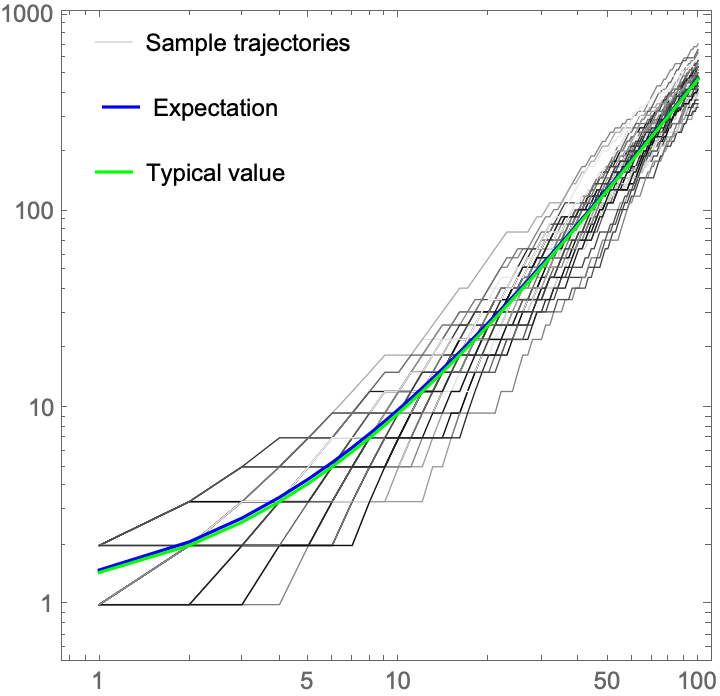
\includegraphics[width=0.9\textwidth]{./sample-trajectories.png}
\end{center}
\captionof{figure}{\small \helveticanarrow \label{fig-trajectories}  Some sample trajectories for $\eta=\frac{1}{2}$ with $g=\frac{3}{2}$ and $r=\frac{1}{2}$.}
\end{Figure}

\bibliographystyle{plain}
\bibliography{refs}


\end{multicols}
\end{document}
